\documentclass{article}
\usepackage{graphicx}

\begin{document}

\begin{figure*}[t!]
\centering
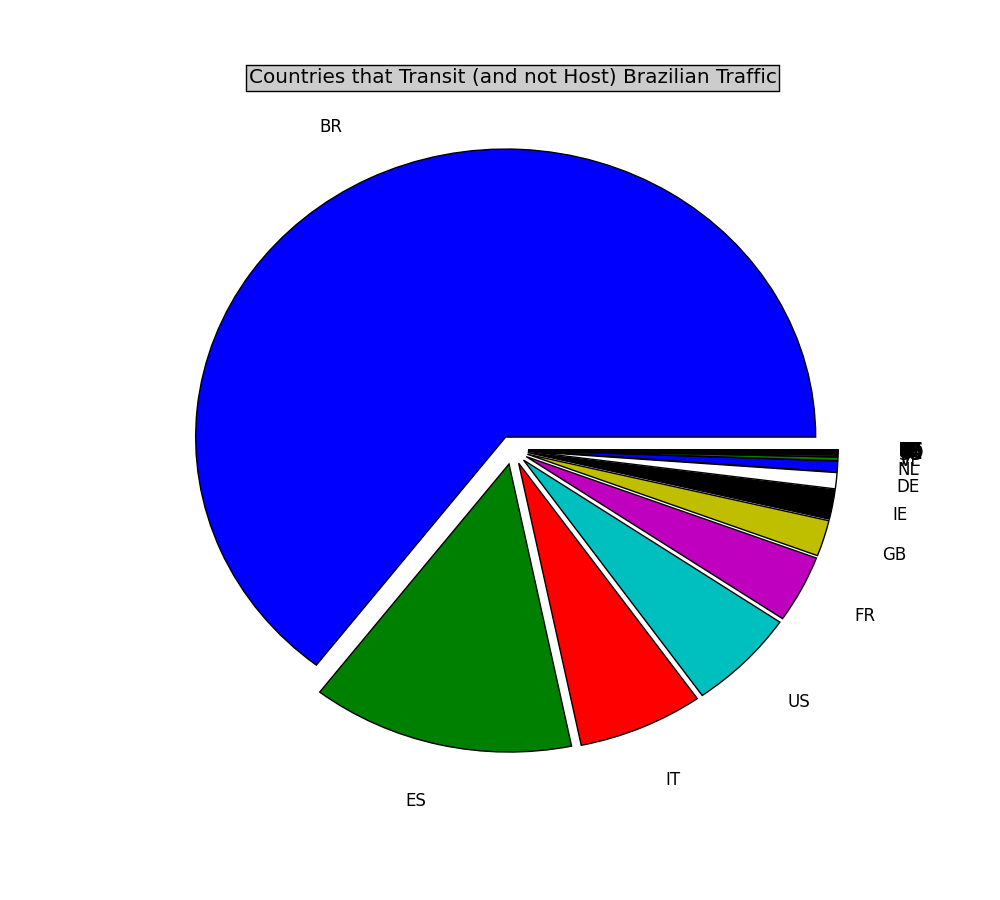
\includegraphics[width=1\textwidth]{paper/figures/brazil_transit}
\caption{The number of paths originating in Brazil that transit (and are not hosted in) Brazil.}
\label{fig:host}
\end{figure*} 

\begin{figure*}[t!]
\centering
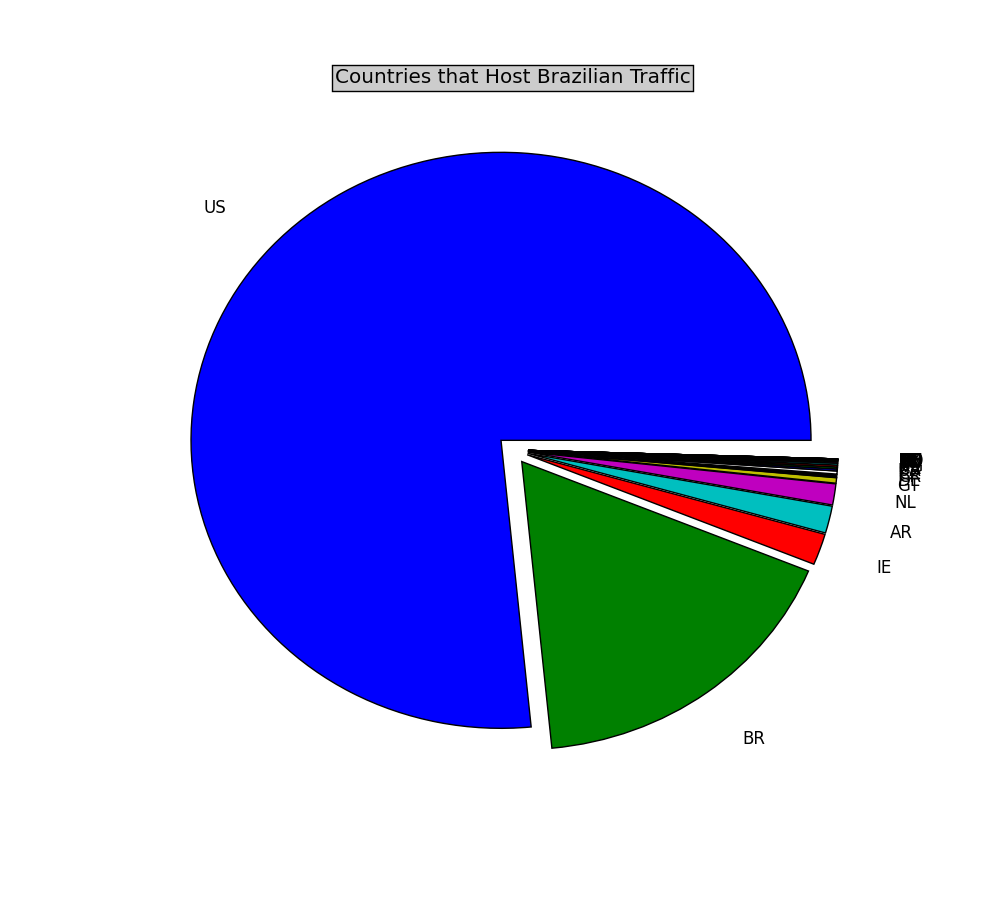
\includegraphics[width=1\textwidth]{paper/figures/brazil_host}
\caption{The number of paths originating in Brazil that are hosted in Brazil.}
\label{fig:host}
\end{figure*} 

\begin{figure*}[t!]
\centering
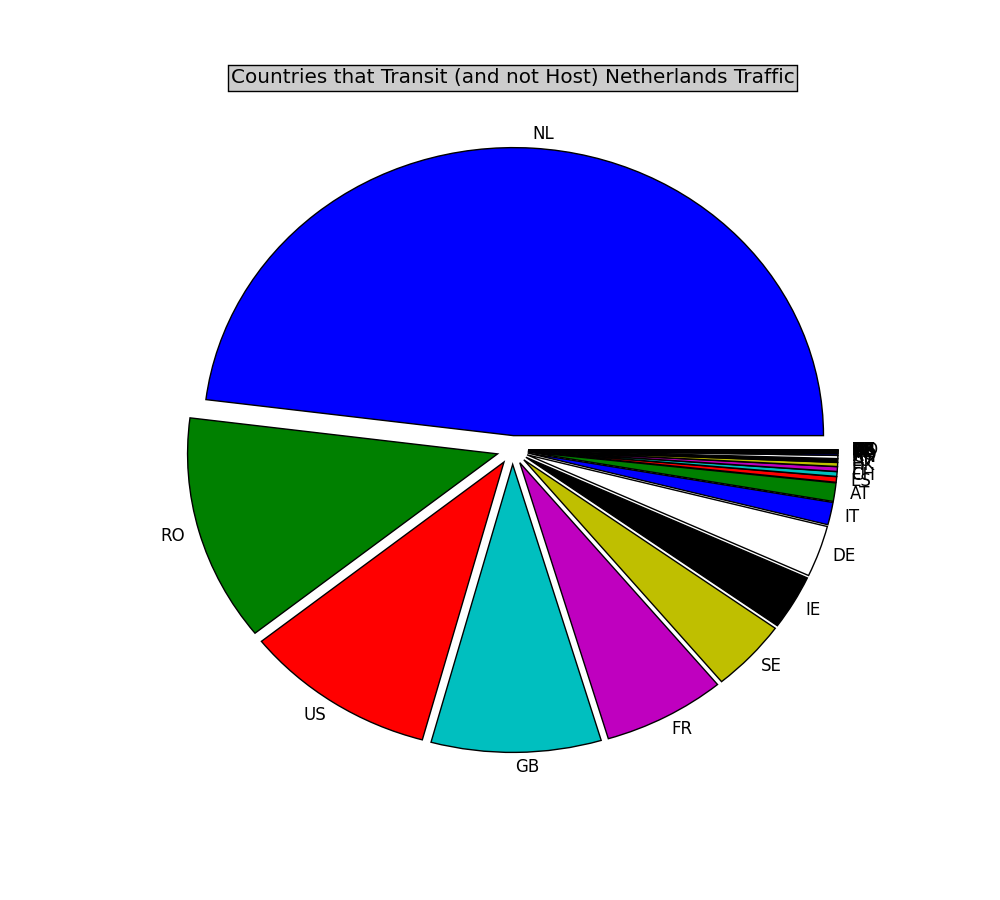
\includegraphics[width=1\textwidth]{paper/figures/netherlands_transit}
\caption{The number of paths originating in Netherlands that transit (and are not hosted in) Netherlands.}
\label{fig:host}
\end{figure*} 

\begin{figure*}[t!]
\centering
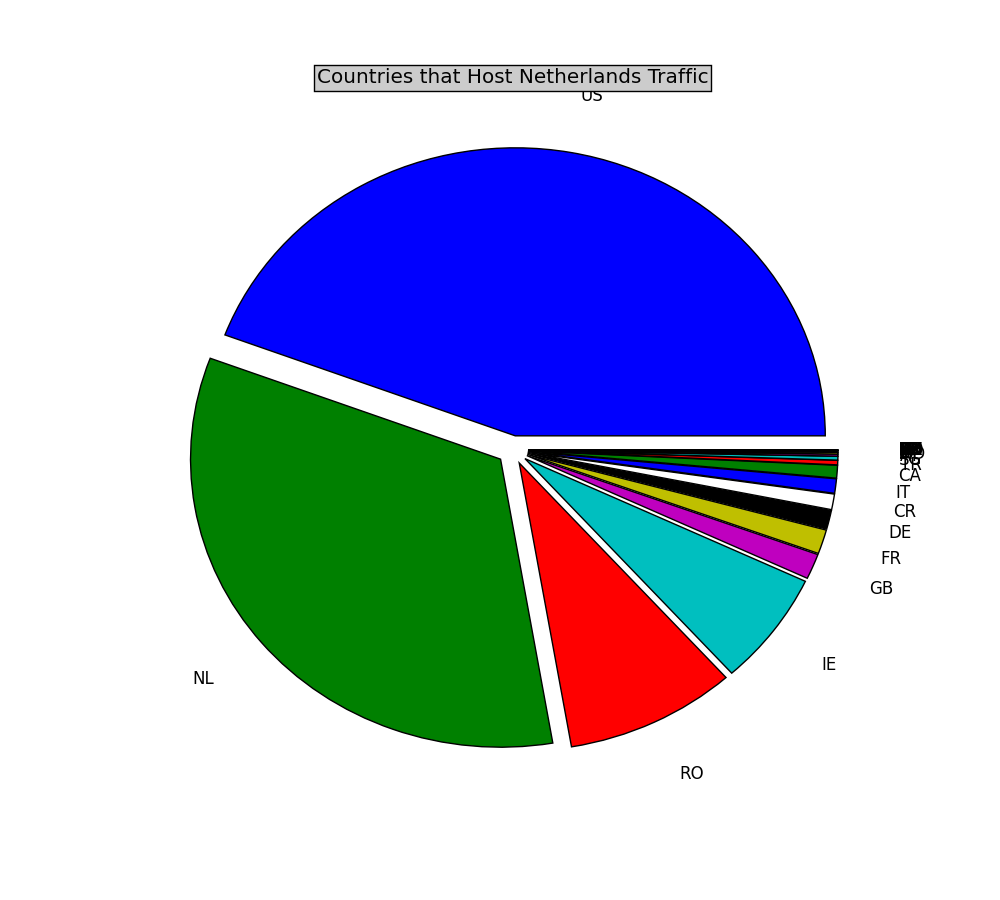
\includegraphics[width=1\textwidth]{paper/figures/netherlands_host}
\caption{The number of paths originating in Netherlands that are hosted in Netherlands.}
\label{fig:host}
\end{figure*} 

\begin{figure*}[t!]
\centering
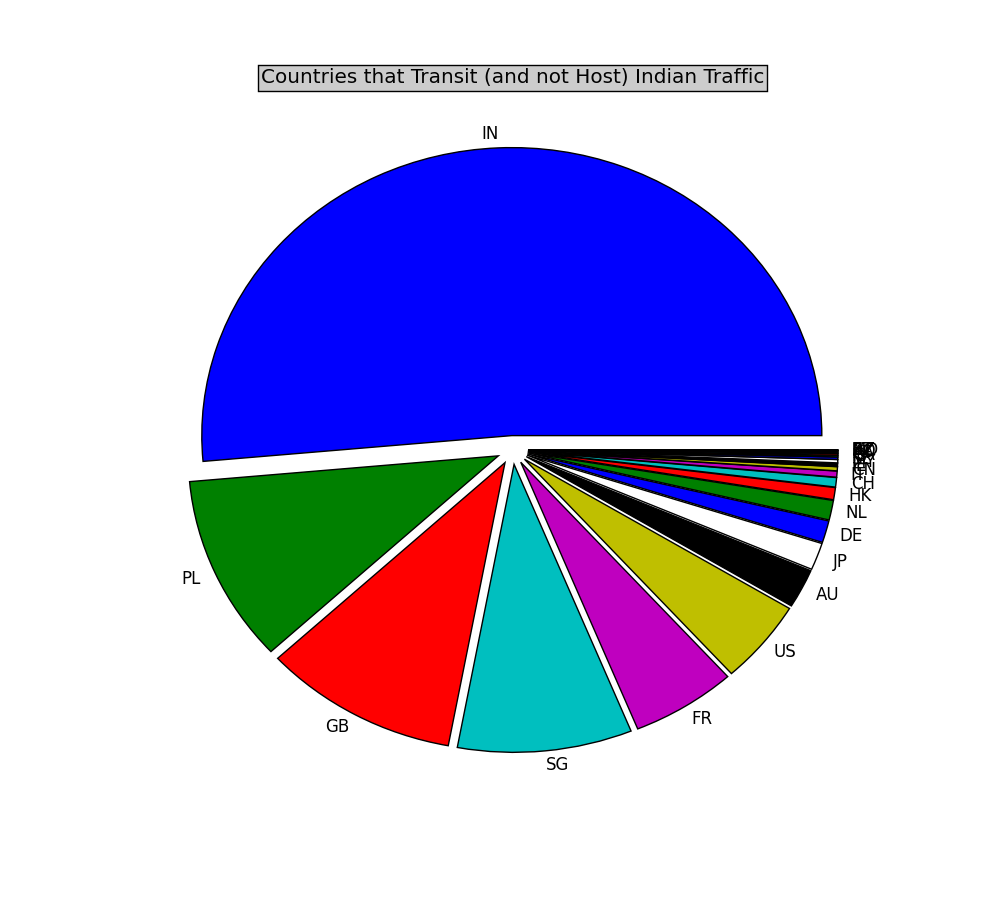
\includegraphics[width=1\textwidth]{paper/figures/india_transit}
\caption{The number of paths originating in India that transit (and are not hosted in) India.}
\label{fig:host}
\end{figure*} 

\begin{figure*}[t!]
\centering
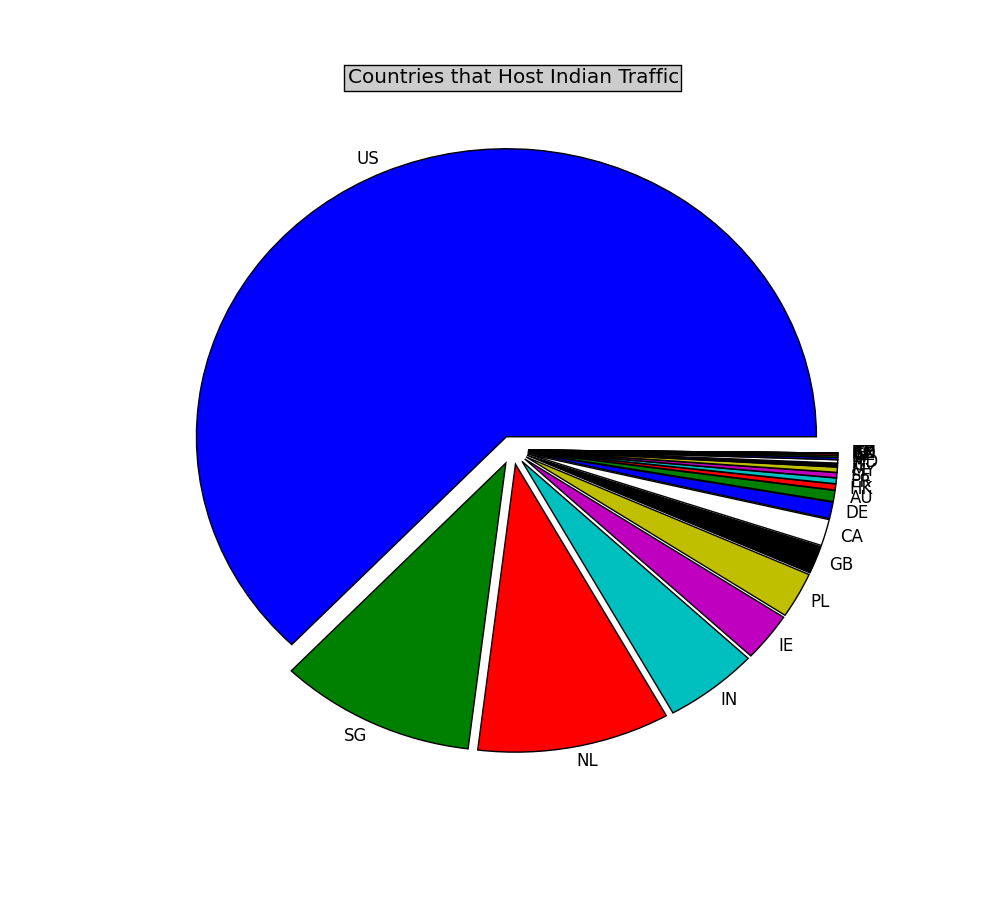
\includegraphics[width=1\textwidth]{paper/figures/india_host}
\caption{The number of paths originating in India that are hosted in India.}
\label{fig:host}
\end{figure*} 

\begin{figure*}[t!]
\centering
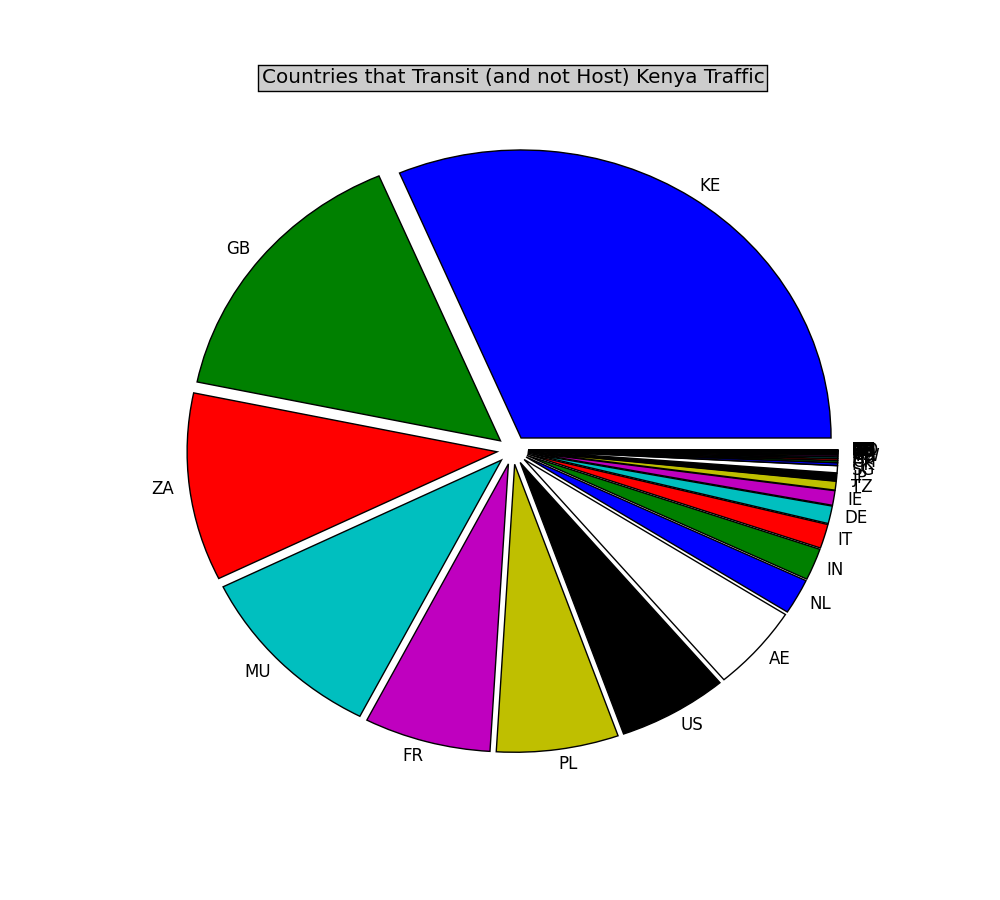
\includegraphics[width=1\textwidth]{paper/figures/kenya_transit}
\caption{The number of paths originating in Kenya that transit (and are not hosted in) Kenya.}
\label{fig:host}
\end{figure*} 

\begin{figure*}[t!]
\centering
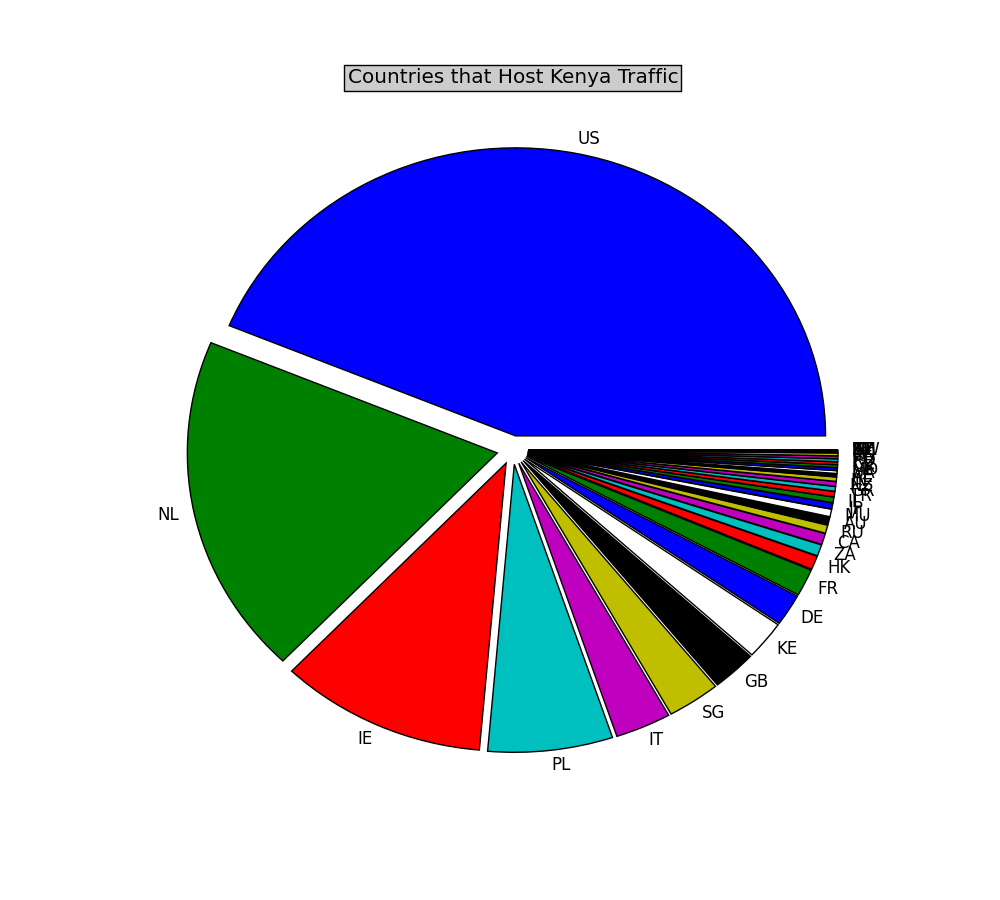
\includegraphics[width=1\textwidth]{paper/figures/kenya_host}
\caption{The number of paths originating in Kenya that are hosted in Kenya.}
\label{fig:host}
\end{figure*}

\end{document}
